\documentclass{beamer}

\beamertemplatenavigationsymbolsempty

\usetheme{default}
\usecolortheme{dolphin}

\usepackage{graphicx}
\usepackage{caption}
\usepackage{tikz}
\usepackage{dsfont}
\usepackage{siunitx}
\usepackage{booktabs}
\usepackage[labelformat=empty]{caption} 
\usetikzlibrary{shapes,arrows}

% Define block styles
\tikzstyle{decision} = [diamond, draw, fill=blue!20, text width=4.5em, text badly centered, node distance=3cm, inner sep=0pt]
\tikzstyle{block} = [rectangle, draw, fill=blue!20, text width=5em, text centered, rounded corners, minimum height=4em]
\tikzstyle{line} = [draw, -latex']
\tikzstyle{cloud} = [draw, ellipse,fill=red!20, node distance=3cm, minimum height=2em]

\setbeamerfont{caption}{size=\tiny}

\begin{document}

\title[Plant Detection and State Classification]{Plant Detection and
  State Classification with Machine Learning}
\author{Tobias Eidelpes}
\date{March 12, 2024}

\begin{frame}
  \maketitle
\end{frame}

\section{Introduction}

\begin{frame}
  \frametitle{Problem Statement}
  \begin{itemize}
    \setlength{\itemsep}{1.1\baselineskip}
  \item Automated detection of water stress \pause
  \item Automated watering of household plants \pause
  \item Decision-making \emph{in the field} \pause
  \item No research so far in this context
  \end{itemize}
\end{frame}

\begin{frame}
  \frametitle{Research Questions}
  \begin{enumerate}
    \setlength{\itemsep}{1.1\baselineskip}
  \item How well does the model work in theory and how well in
    practice? \pause
  \item What are possible reasons for it to work/not work? \pause
  \item What are possible improvements to the system in the future?
  \end{enumerate}
\end{frame}

\section{Methodological Approach}

\begin{frame}
  \frametitle{Methods}
  \begin{columns}[c]
    \column{.5\textwidth}
    \begin{enumerate}
      \setlength{\itemsep}{1.1\baselineskip}
    \item Literature Review
    \item Dataset Curation
    \item Model Training
    \item Optimization
    \item Deployment
    \item Evaluation
    \end{enumerate}
    \column{.5\textwidth}
    \begin{center}
      \includegraphics[width=\textwidth]{graphics/wilted\_007.jpg}
    \end{center}
  \end{columns}
\end{frame}

\section{Prototype Design}

\begin{frame}
  \frametitle{Prototype Design: Requirements} \pause
  \begin{itemize}
    \setlength{\itemsep}{1.1\baselineskip}
  \item Detect and Classify \pause
  \item Publish Results via REST-API \pause
  \item Reasonable Inference Time \pause
  \item Reasonable Model Performance
  \end{itemize}
\end{frame}

\begin{frame}
  \frametitle{Prototype Design}
  \begin{figure}[htbp]
    \centerline{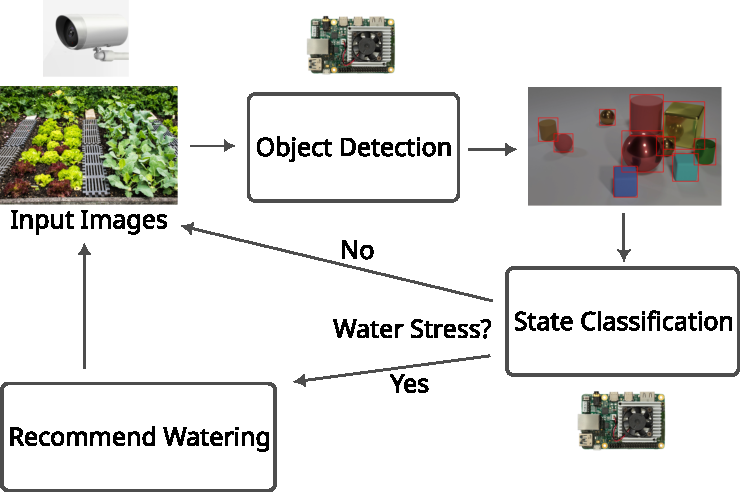
\includegraphics[width=0.9\textwidth]{graphics/setup.pdf}}
    \label{fig:design}
  \end{figure}
\end{frame}

\section{Prototype Implementation}

\begin{frame}
  \frametitle{Prototype Implementation: YOLOv7n}
  \begin{minipage}[bt]{.49\textwidth}
    \begin{itemize}
      \setlength{\itemsep}{1.1\baselineskip}
    \item Pretrained on COCO
    \item OID classes \emph{Houseplant} and \emph{Plant}
    \item Training Set
      \begin{itemize}
      \item \num{79204} images
      \item \num{284130} bounding boxes
      \end{itemize}
    \item Validation Set
      \begin{itemize}
      \item \num{3091} images
      \item \num{4092} bounding boxes
      \end{itemize}
    \end{itemize}
  \end{minipage}
  \begin{minipage}[bt]{.49\textwidth}
    \vspace{.5cm}
    \begin{figure}
      \begin{center}
        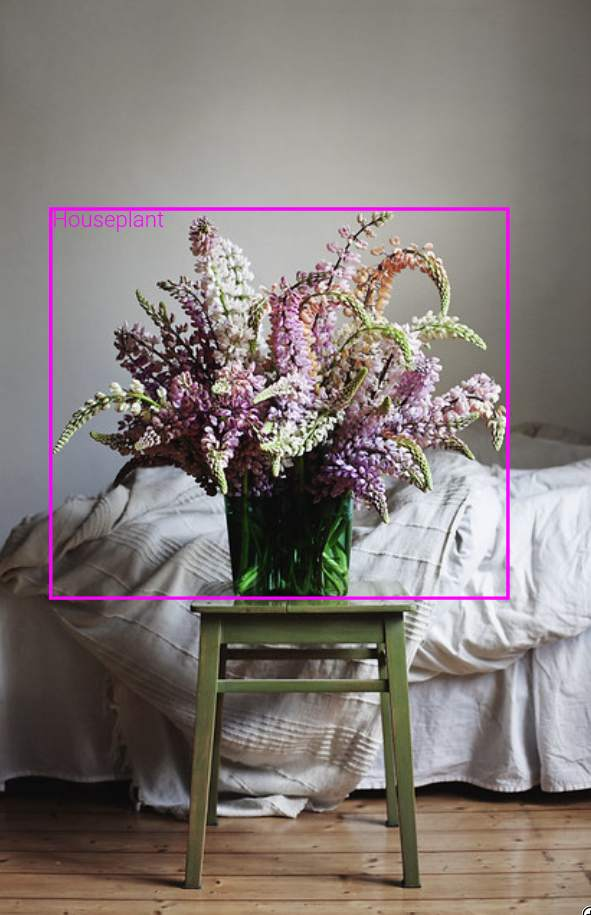
\includegraphics[width=.85\textwidth]{graphics/houseplant.jpg}
        \caption{Earthy Tones For Fallsurlevif by Flickr User decor8
          under CC BY 2.0}
      \end{center}
    \end{figure}
  \end{minipage}
\end{frame}

\begin{frame}
  \frametitle{Prototype Implementation: YOLOv7n}
  \begin{figure}[htbp]
    \begin{center}
      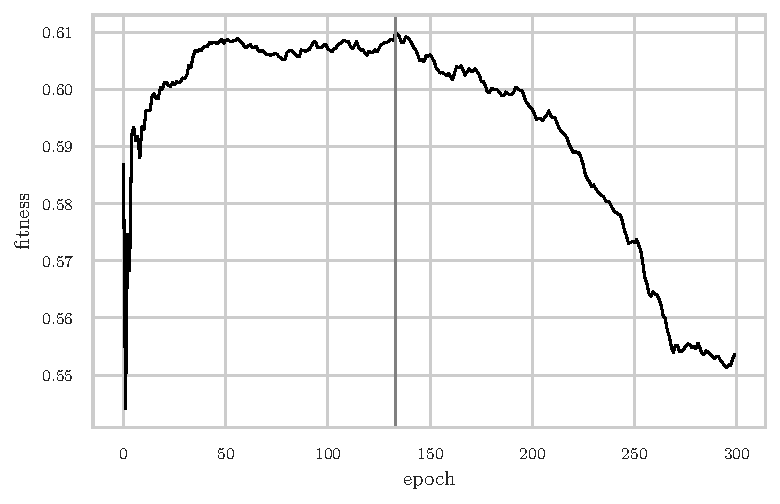
\includegraphics[width=\textwidth]{graphics/model_fitness.pdf}
    \end{center}
  \end{figure}
\end{frame}

\begin{frame}
  \frametitle{Prototype Implementation: YOLOv7n}
  \begin{figure}[htbp]
    \begin{center}
      \includegraphics[width=\textwidth]{graphics/val\_box\_obj\_loss.pdf}
    \end{center}
  \end{figure}
\end{frame}

\begin{frame}
  \frametitle{YOLOv7n Hyperparameter Optimization} \pause
  \begin{itemize}
    \setlength{\itemsep}{1.1\baselineskip}
  \item Mutate 26 out of 30 hyperparameters \pause
  \item Parent chosen randomly from top five previous generations \pause
  \item 3 epochs per iteration \pause
  \item 87 iterations \pause
  \item Best with 0.6076 fitness
  \end{itemize}
\end{frame}

\begin{frame}
  \frametitle{YOLOv7n Hyperparameter Optimization}
  \begin{figure}[htbp]
    \begin{center}
      \includegraphics[width=\textwidth]{graphics/model_fitness\_final.pdf}
    \end{center}
  \end{figure}
\end{frame}

\begin{frame}
  \frametitle{Prototype Implementation: ResNet-50}
  \begin{minipage}[bt]{.49\textwidth}
    \begin{itemize}
      \setlength{\itemsep}{1.1\baselineskip}
    \item Pretrained on ImageNet
    \item Training Set
      \begin{itemize}
      \item \num{384} healthy
      \item \num{384} stressed
      \end{itemize}
    \item Validation Set
      \begin{itemize}
      \item \num{68} healthy
      \item \num{68} stressed
      \end{itemize}
    \end{itemize}
  \end{minipage}
  \begin{minipage}[bt]{.49\textwidth}
    \begin{center}
      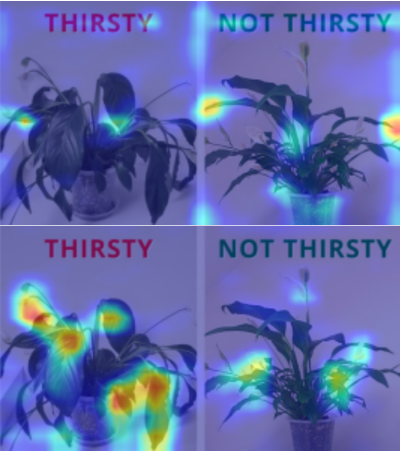
\includegraphics[width=\textwidth]{graphics/classifier-cam-cropped.pdf}
    \end{center}
  \end{minipage}
\end{frame}

\begin{frame}
  \frametitle{Prototype Implementation: ResNet-50 Accuracy}
  \begin{figure}[htbp]
    \begin{center}
      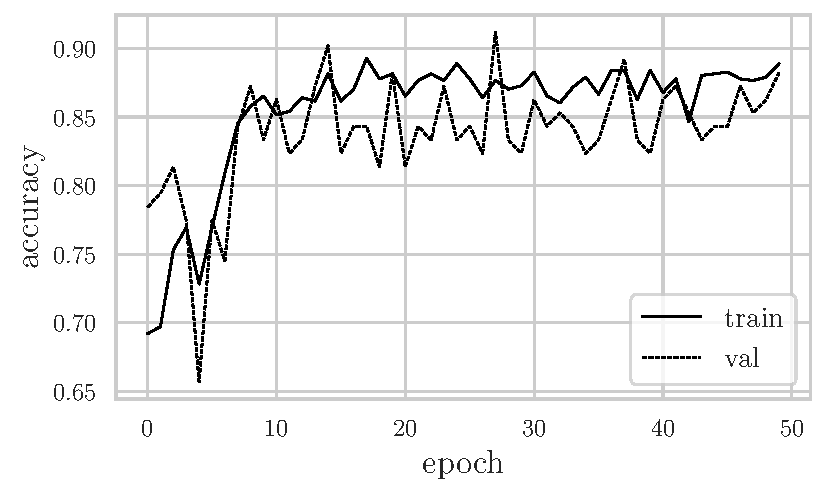
\includegraphics[width=\textwidth]{graphics/classifier-metrics-acc.pdf}
      \caption{\normalsize Maximum validation accuracy of 0.9118 at epoch 27}
    \end{center}
  \end{figure}
\end{frame}

\begin{frame}
  \frametitle{Prototype Implementation: ResNet-50 Loss}
  \begin{figure}[htbp]
    \begin{center}
      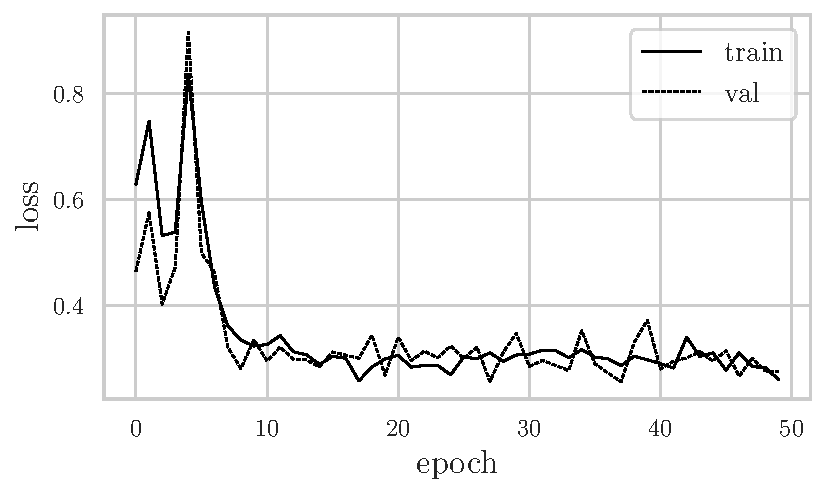
\includegraphics[width=\textwidth]{graphics/classifier-metrics-loss.pdf}
    \end{center}
  \end{figure}
\end{frame}

\begin{frame}
  \frametitle{ResNet-50 Hyperparameter Optimization}
  \begin{itemize}
    \setlength{\itemsep}{1.1\baselineskip}
  \item Random search \pause
  \item 10 epochs per iteration \pause
  \item 138 iterations \pause
  \item Best with 0.9783 $\mathrm{F}_{1}$-score 
  \end{itemize}
\end{frame}

\begin{frame}
  \frametitle{ResNet-50 Hyperparameter Optimization}
  \begin{figure}[htbp]
    \centerline{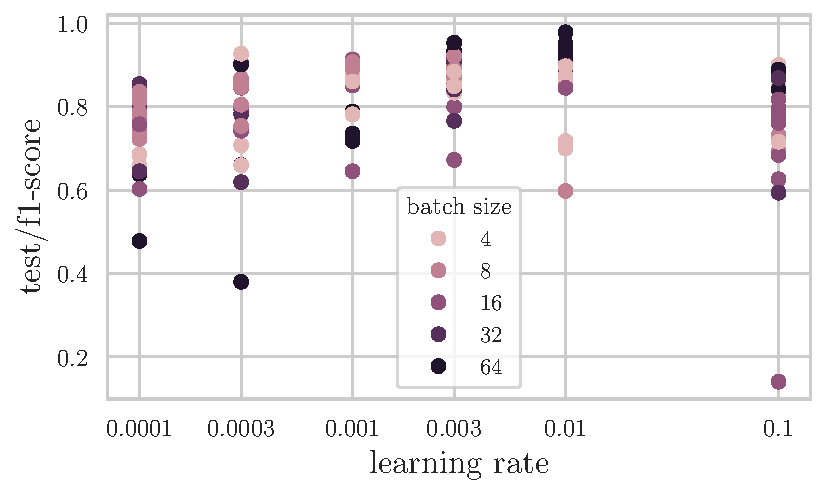
\includegraphics[width=\textwidth]{graphics/classifier-hyp-metrics.pdf}}
    \caption{\normalsize Learning rate and batch size effect on
      $\mathrm{F}_{1}$-score}
  \end{figure}
\end{frame}

\section{Evaluation}

\begin{frame}
  \frametitle{YOLOv7n Evaluation}
  \begin{itemize}
    \setlength{\itemsep}{1.1\baselineskip}
  \item Test Set
    \begin{itemize}
    \item \num{9000} images
    \item \num{12238} bounding boxes \pause
    \end{itemize}
  \end{itemize}
  \begin{table}[h]
    \centering
    \begin{tabular}{lrrrr}
      \toprule
      {} &  Precision &    Recall &  $\mathrm{F}_1$-score &  Support \\
      \midrule
      Plant        &   \num{0.5476} &  \num{0.7379} &  \num{0.6286} &  \num{12238} \\
      \bottomrule
    \end{tabular}
    \caption{\scriptsize Results for the non-optimized object detection model}
    \label{tab:yolo-metrics}
  \end{table}
  \begin{table}[h]
    \centering
    \begin{tabular}{lrrrr}
      \toprule
      {} &  Precision &    Recall &  $\mathrm{F}_1$-score &  Support \\
      \midrule
      Plant        &   \num{0.6334} &  \num{0.7028} &  \num{0.6663} &  \num{12238} \\
      \bottomrule
    \end{tabular}
    \caption{\scriptsize Results for the optimized object detection model}
    \label{tab:yolo-metrics-hyp}
  \end{table}
\end{frame}

\begin{frame}
  \frametitle{ResNet-50 Evaluation}
  \begin{center}
    \begin{figure}[htbp]
      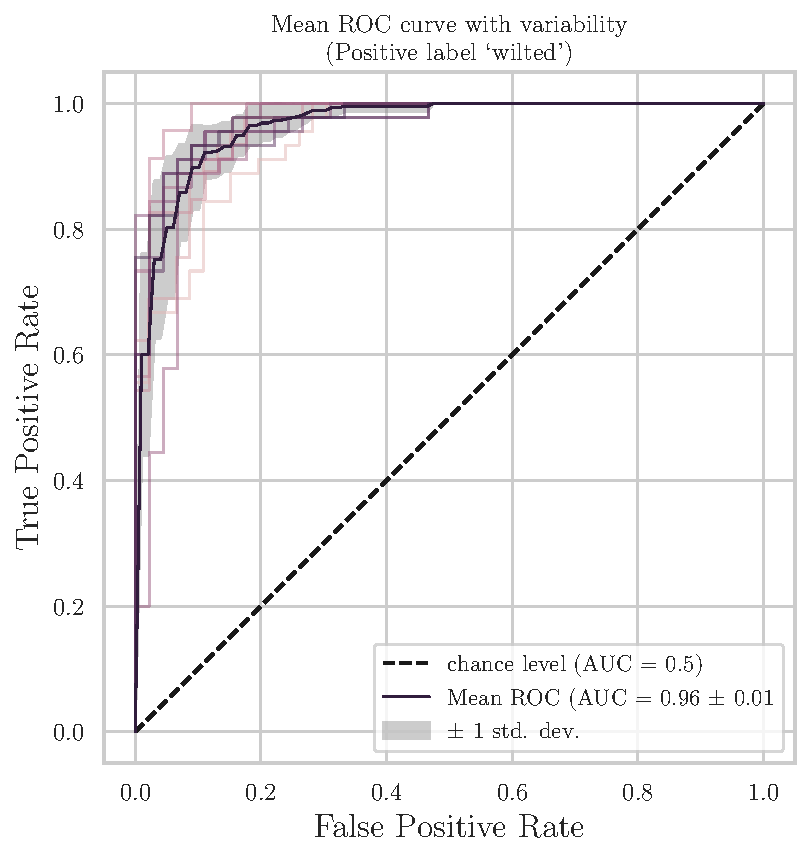
\includegraphics[width=0.65\textwidth]{graphics/classifier-hyp-folds.pdf}
      \caption{\scriptsize ROC curves and AUC for classifier 10-fold
        cross-validation}
    \end{figure}
  \end{center}
\end{frame}

\begin{frame}
  \frametitle{Aggregate Model Evaluation}
  \begin{itemize}
    \setlength{\itemsep}{1.1\baselineskip}
  \item Pre-annotated Test Set
    \begin{itemize}
    \item \num{640} images
    \item \num{766} bounding boxes healthy
    \item \num{494} bounding boxes stressed \pause
    \end{itemize}
  \item Non-optimized model $\mathrm{mAP} = 0.3581$ \pause
  \item Optimized model $\mathrm{mAP} = 0.3838$
  \end{itemize}
\end{frame}

\section{Conclusion}

\begin{frame}
  \frametitle{Limitations and Conclusions}
  \begin{itemize}
    \setlength{\itemsep}{0.75\baselineskip}
  \item I am \emph{not} an expert labeler! \pause
  \item Object detection performs well (mAP 0.5727) \pause
  \item Optimized detector worse than non-optimized \pause
  \item Inconsistent ground truth \pause
  \item Robust classification
  \end{itemize}
\end{frame}

\begin{frame}
  \frametitle{Research Questions Revisited}
  \begin{enumerate}
    \setlength{\itemsep}{1.1\baselineskip}
  \item How well does the model work in theory and how well in practice? \pause
    \begin{itemize}
    \item Plant detection comparable to benchmarks \pause
    \item Impressive stress classification \pause
    \end{itemize}
  \item What are possible reasons for it to work/not work? \pause
    \begin{itemize}
    \item Dataset curation \pause
    \end{itemize}
  \item What are possible improvements to the system in the future? \pause
    \begin{itemize}
    \item Use more computational resources \pause
    \item Expert labeling
    \end{itemize}
  \end{enumerate}
\end{frame}

\begin{frame}
	\centering
	\Large
	Thank you for your attention!
\end{frame}

\begin{frame}
  \frametitle{ResNet-50 CAM}
  \begin{figure}[htbp]
    \centerline{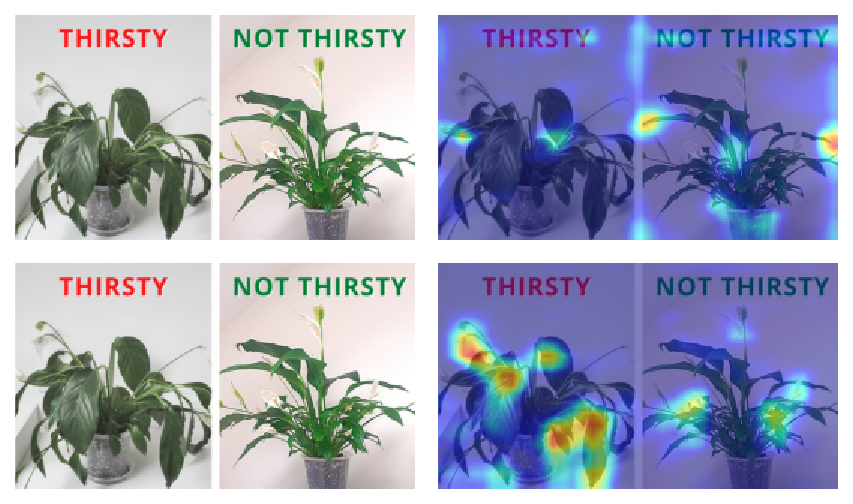
\includegraphics[width=0.9\textwidth]{graphics/classifier-cam.pdf}}
    \caption[]{\label{fig:classifier-cam} Top-right: CAM for
      \emph{healthy}. Bot-right: CAM for \emph{stressed}}
  \end{figure}
\end{frame}

\begin{frame}
  \frametitle{Aggregate Model Evaluation}
  \begin{table}
    \centering
    \begin{tabular}{lrrrr}
      \toprule
      {} &  Precision &  Recall &  $\mathrm{F}_{1}$-score &  Support \\
      \midrule
      Healthy      &      \num{0.665} &   \num{0.554} &     \num{0.604} &    \num{766} \\
      Stressed     &      \num{0.639} &   \num{0.502} &     \num{0.562} &    \num{494} \\
      Weighted Avg &      \num{0.655} &   \num{0.533} &     \num{0.588} &   \num{1260} \\
      \bottomrule
    \end{tabular}
    \caption{Metrics for the non-optimized aggregate model}
    \label{tab:model-metrics}
  \end{table}
  \begin{table}
    \centering
    \begin{tabular}{lrrrr}
      \toprule
      {} &  Precision &  Recall &  $\mathrm{F}_{1}$-score &  Support \\
      \midrule
      Healthy      &      0.711 &   0.555 &     0.623 &    766 \\
      Stressed     &      0.570 &   0.623 &     0.596 &    494 \\
      Weighted Avg &      0.656 &   0.582 &     0.612 &   1260 \\
      \bottomrule
    \end{tabular}
    \caption{Metrics for the optimized aggregate model}
    \label{tab:model-metrics-hyp}
  \end{table}
\end{frame}


\end{document}
%%% Local Variables:
%%% mode: LaTeX
%%% TeX-master: t
%%% End:
